% Figure 1: Local Closure vs Global Non-Closure
% Standalone TikZ figure for BP3
\documentclass[tikz,border=5pt]{standalone}
\usepackage{tikz}
\usetikzlibrary{shapes.geometric,arrows.meta,positioning,decorations.pathmorphing,calc}

\begin{document}
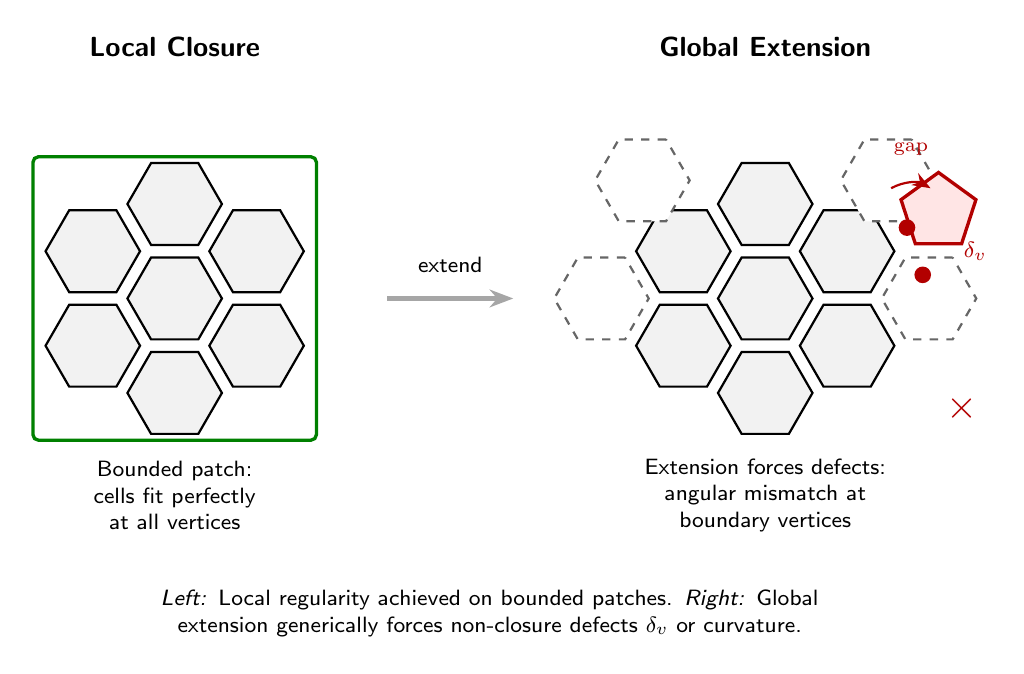
\begin{tikzpicture}[
    cell/.style={regular polygon, regular polygon sides=6, minimum size=1.2cm, draw=black, thick, fill=gray!10},
    defectcell/.style={regular polygon, regular polygon sides=6, minimum size=1.2cm, draw=black!60, thick, fill=white, dashed},
    gapcell/.style={regular polygon, regular polygon sides=5, minimum size=1cm, draw=red!70!black, very thick, fill=red!10},
    label/.style={font=\small\sffamily},
    annotation/.style={font=\footnotesize\sffamily, align=center},
    arrow/.style={-{Stealth[length=3mm]}, thick, gray!70}
]

% === LEFT PANEL: Local Closure ===
\begin{scope}[shift={(-4.5,0)}]
    % Title
    \node[annotation, font=\sffamily\bfseries] at (0,3.2) {Local Closure};

    % Central hexagonal patch (honeycomb-like)
    \node[cell] (c0) at (0,0) {};
    \node[cell] (c1) at (1.04,0.6) {};
    \node[cell] (c2) at (1.04,-0.6) {};
    \node[cell] (c3) at (0,-1.2) {};
    \node[cell] (c4) at (-1.04,-0.6) {};
    \node[cell] (c5) at (-1.04,0.6) {};
    \node[cell] (c6) at (0,1.2) {};

    % Perfect fit indicator
    \draw[green!50!black, very thick, rounded corners=2pt] (-1.8,-1.8) rectangle (1.8,1.8);

    % Checkmark
    \node[green!50!black, font=\Large] at (1.4,1.4) {\checkmark};

    % Annotation
    \node[annotation, text width=3.5cm] at (0,-2.5) {Bounded patch:\\cells fit perfectly\\at all vertices};
\end{scope}

% === ARROW ===
\draw[arrow, line width=1.5pt] (-1.8,0) -- (-0.2,0);
\node[annotation, above] at (-1,0.2) {extend};

% === RIGHT PANEL: Global Extension with Defects ===
\begin{scope}[shift={(3,0)}]
    % Title
    \node[annotation, font=\sffamily\bfseries] at (0,3.2) {Global Extension};

    % Core cells
    \node[cell] (d0) at (0,0) {};
    \node[cell] (d1) at (1.04,0.6) {};
    \node[cell] (d2) at (1.04,-0.6) {};
    \node[cell] (d3) at (0,-1.2) {};
    \node[cell] (d4) at (-1.04,-0.6) {};
    \node[cell] (d5) at (-1.04,0.6) {};
    \node[cell] (d6) at (0,1.2) {};

    % Attempted extension - with gaps/mismatches
    \node[defectcell] (e1) at (2.08,0) {};
    \node[defectcell] (e2) at (1.56,1.5) {};
    \node[defectcell] (e3) at (-1.56,1.5) {};
    \node[defectcell] (e4) at (-2.08,0) {};

    % Gap/defect region (pentagonal - wrong shape)
    \node[gapcell] (gap1) at (2.2,1.1) {};

    % Defect markers
    \fill[red!70!black] (1.8,0.9) circle (3pt);
    \fill[red!70!black] (2.0,0.3) circle (3pt);
    \node[red!70!black, font=\footnotesize\bfseries, right] at (2.4,0.6) {$\delta_v$};

    % Angular deficit annotation
    \draw[red!70!black, thick, -{Stealth}] (1.6,1.4) arc (120:60:0.5);
    \node[red!70!black, font=\scriptsize, above] at (1.85,1.7) {gap};

    % Warning indicator
    \node[red!70!black, font=\Large] at (2.5,-1.4) {$\times$};

    % Annotation
    \node[annotation, text width=4cm] at (0,-2.5) {Extension forces defects:\\angular mismatch at\\boundary vertices};
\end{scope}

% === Bottom annotation ===
\node[annotation, text width=10cm, align=center] at (-0.5,-4) {
\textit{Left:} Local regularity achieved on bounded patches.
\textit{Right:} Global extension generically forces non-closure defects $\delta_v$ or curvature.
};

\end{tikzpicture}
\end{document}
